\chapter{Peatlands}\label{ch:peatlands}
\chapterauthor {Rebecca Chung and Christine Chan\footnote{Statement of Contributions: }}

\section{Introduction}

\subsection{Peatlands}

Peatland are wetlands that are dominated by peat forming plants that originate from biological processes. Peatland make up 3\% of the earth and are mostly found in East Asia, Southeast Asia, the Caribbean and Central America, South America and southern Africa \citep{strack2008peatlands}. Peatland globally have a  significant role in storage of soil carbon. 

Forest tropical peatlands in Southeast Asia store 42,000 million metric tonnes (Mt) of soil carbon. The stability of this pool is at risk due to the recent decades of deforestation, drainage, and fire. 

Peatland are vital when it comes to biological process because of the immense amount of carbon storage you can find in the systems, carbon dioxide sink, and atmospheric methane point. Peatland contribute small portion to the emission of CH4  and N2O but the sequestration of CO2 are far greater \citep{strack2008peatlands}. The Greenhouse gases properties of peatland is a shifting role that depends on the peatlands ecology, hydrology, climate, and climate change. The CO2 emission at times can be so great that the peatland can change from a sink to a source at times. Changing vegetation can contribute to shifts in carbon sequestration due to elevated water and production.

The major actors to disturbing Peatlands natural processes  are agriculture, forestry, peat fuel extraction, and horticulture.  Indonesia 3.7 million hectares of peatland are drained and being used for agriculture. This dramatically decrease C fixation capacity and threatened greenhouse gas emissions

Peatland can serve a very powerful asset to assuring carbon sequestration and mitigate emissions in the region.

Three components have been found to contribute in the change of carbon flux between soil and atmosphere




Southeast Asia is home to most of the world's tropical peat. In these humid conditions, peat is created and conserved in the ecosystems because peat relies on a consistent source of water year-round through rainfull or humidity. Peat, the accumulation of partly decomposed vegetable matter, makes up a peatland, which is characterized as a type of wetland with peat soil and a wetland habitat. 

Palm oil, an edible vegetable oil from the fruit of an oil palm plant, grows well year-round in the climate of Southeast Asia and on the region's peatlands. An intensified global demand for palm oil can be very harmful to public health and the climate \citep{knitr2013}. International corporations rely on palm oil for the creation of different cosmetics and processed foods. These corporations therefore place enormous pressure on local farmers to transition from subsistence mixed farming to growing exclusively palm oil. To create space for palm oil plantations, local farmers in Southeast Asia use an agricultural method called slash-and-burn, in which they burn the peatlands for large-scale palm oil plantations. Because these fires are unregulated and difficult to control, air pollution in the region has intensified. Many of the inhabitants in Southeast Asia are familiar with what is called the Southeast Asia Haze. The quality of air in Southeast Asia has deteriorated severely recently. Coinciding with a fall in air and water quality in the region is an expontential growth in demand for palm oil. 

\begin{figure}[!ht]
  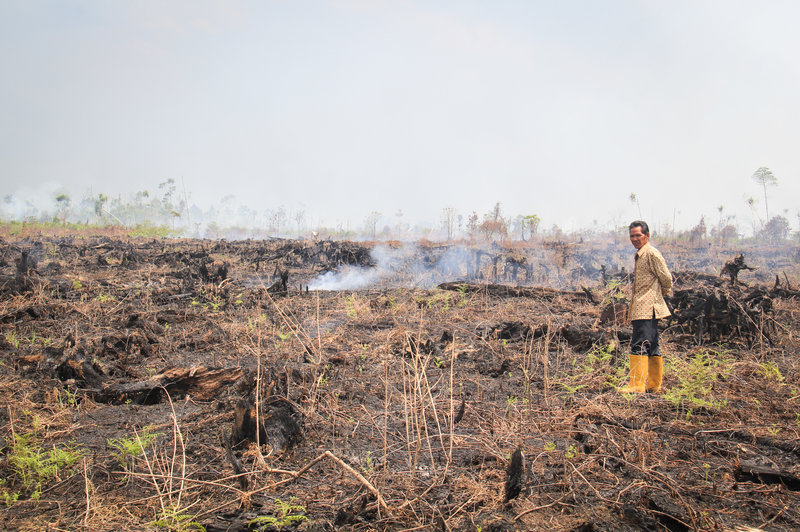
\includegraphics[width=\linewidth]{arifpicture.jpg}
  \caption{NPR captured a picture of the farmer Arif Subandi and the burnt peatlands near his home.}
  \label{fig:arifpicture}
\end{figure}

Beyond simply deforestation, the problem of using the slash-and-burn method on peatlands specifically is that the nature of peat makes it incredibly difficult to put out the prescribed fires. As a result, the fires burn for much longer and create much more smoke than if they were prescribed on different types of forest lands. These fires can quickly grow out of control and spread into protected forests. Fires on peatlands can then create environmental and health hazards for the local communities as well as have lasting impacts on global climate because of the magnitude of the carbon emissions. In this chapter, we will investigate the anthropogenic impacts on the environment and global climate within the context of peatlands in Southeast Asia. 

NPR covered the story of a farmer on one of Indonesia's major islands who illustrates the ecological importance and fragility of peatlands. Arif Subandi who lives in Borneo lost his family's farmland to fires on peatlands that were caused by local companies trying to use the land to create palm oil plantations (figure \ref{fig:arifpicture}). In the past, a lack of legal enforcement of bans on peatland fires and deforestation in protected areas has forced out indigenous people who live and rely on peatland ecosystems to survive. The creation of palm oil plantations for global supply chains threaten the livelihoods of farmers like Arif Subandi. Arif faces physical threats from different corporations, whether motorcycle corporations or palm oil corporations, to move off the land despite having cultivated it for many generations. 

In Indonesia, specifically, the lived experiences of people who live near peatlands illustrate how damaging certain agricultural techniques can be to the livelihoods of rural people and the natural environment. Because Indonesia produces much of the world's palm oil, it can be a useful case study in understanding peatlands and anthropogenic impacts to peatlands in the twenty-first century. 

\section{What is peat?}

Peat is an organic fuel consisting of partially or completely decomposed organic matter. The organic matter is primarly different kinds of plants and is composed when this organic material has accumulated in a water-saturated environment. The plants that form peatlands tend to be more resistant to decay than ordinary plant litter and one example of a plant that commonly forms peatlands is the Sphagnum species \citep{holden2005peatland}. Sphagnum is a genus of about 380 species of mosses that are called peat mosses. Both living and dead Sphagnum mosses can hold enormous masses of water. Because these plants are more resistant to decay than plants in other ecosystems, the immersion of water combined with this slow rate of decay allows the accumulation of carbon. The ecosystem dynamics in the peatlands are complex. In warm climates, like Southeast Asia, the plant material can decompose more quickly. 

\citet{bridgham2008rapid} puts the amount of carbon in perspective by saying that the global peatland soil-carbon pool is 75 times larger than annual anthropogenic carbon dioxide emissions. With this comparison, it becomes very clear that the need to keep carbon sequestered in the peatlands is extremely important in preventing the release of excess greenhouse gas emissions that could further exacerbate global warming. A peatland's carbon balance can change within the span of a few years. The transition of a peatland from a carbon sink, an ecological reservoir that can absorb and store carbon dioxide from the atmosphere, to a carbon source, which is one that now releases more carbon than it stores.  

Some examples of peatlands across the globe include swamps, muskegs, bogs, fens and moors. In the United States, for example, the swamps and marshes in Florida are examples of peatlands. In Southeast Asia, the more common forms of peatlands are lowland tropical peatlands which are naturally vegetated with a mosaic of specialized closed canopy forests, which refers to a dense growth of trees in which the top branches and leaves form a canopy that light can penetrate very little of to reach the forest floor, linked to local hydrological and nutritional conditions \citep{chokkalingam2005fire}.

See \citet{dennis2005fire}? 

In the wet season, peatlands are flooded by nearby lakes and rivers to depths of up to 3 meters. In the dry season, peatlands can dry out and their water levels drop greatly \citep{chokkalingam2005fire}. Differences in the water supply create differences in what the peatland's soil chemistry, nutrient availability, carbon quality, and the appearance of the plant community composition  Regardless of the type of hydrology in a specific peatland, peatlands can best be categorized as soil-carbon pools. 

\section{How is peat formed?}

\begin{figure}{!ht}
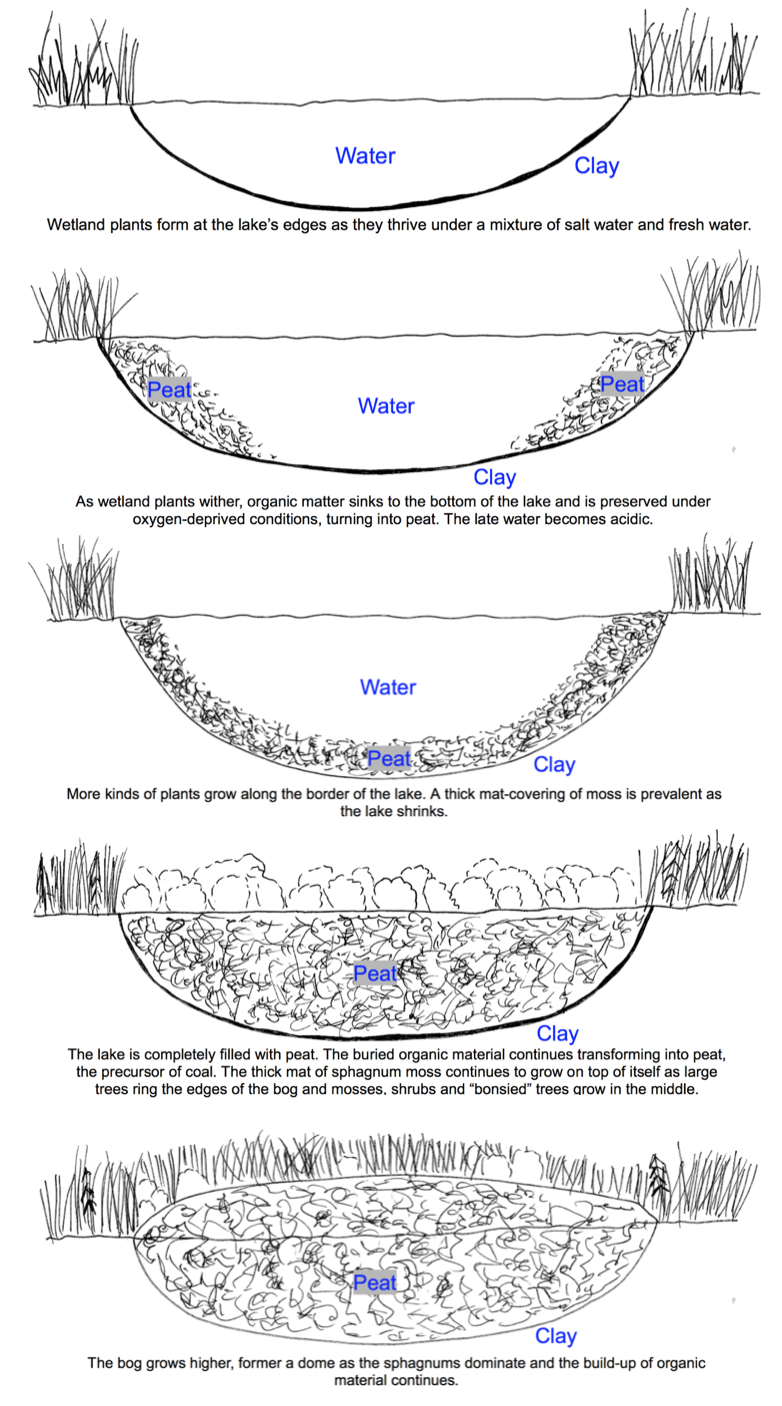
\includegraphics[width=0.5\textwidth]{peatpeat.png}
  \caption{How is peat formed?}
  \label{fig:peatformation}
\end{figure}

Peat decompositions are mostly carried out by microrganisms that use soil organic compounds as energy substrates, and are found across northern North America, northern Europe, western Siberia, Indonesia, and Southeast Asia \citep{rezanezhad2016structure}.

Conditions of near permanent waterlogging, that is, the absence of oxygen in soil, favors accumulation of partially decayed organic matter. This creates long-term ecosystem carbon storage, also known as carbon sinks. In the modern day, these processes are heavily damaged by human activity, such as monoculture farms and logging, and changes in land use, especially in Southeast Asia \citep{page2016line}.

\subsection{Characteristics of peat}

Different peatlands will exhibit vertical movement, either daily or seasonal, based on the water availability at the time, as peat is highly compressible. Peatlands generally swell and shrink when there are changes in water storage, hydraulics, biogeochemistry, and thermal properties. 

Here are some quick facts about peat:
\begin{enumerate}

\item Peat's total porosity exceeds 80 percent! It is also dual-porosity in nature, which increases water flow and solute migration.

\item It is made up of 90 percent of water.

\item In its natural state, peat has a high degree of resistance towards fires, mainly due to a groundwater table within close proximity to the forest floor. However, rising temperatures and decrease in moisture content may reduce its effectiveness.

  \item Compressibility of peat is controlled by its physical properties, including porosity and decomposition. 
  
\end{enumerate}

\subsection{What is carbon storage?}

Tropical peatlands contain up to 90 gigatons of carbon. Most of the carbon that is stored in the peatlands is organic carbon from decomposed plants or plants that are still alive. A small amount of the carbon stored is in an inorganic form, such as in the form of calcium carbonate. Southeast Asia alone has a stock of approximately 69 gigatons \citep{page2016line}. 

Peatlands are a carbon sink. They help regulate global temperatures. Over time, peatlands -- under the right conditions, unencumbered by human activity, can also decrease the amount of carbon dioxide in the atmosphere. Another reason why peatlands are so efficient at creating long-term carbon stores is because heterotrophic respiration, which is a very common form of carbon loss, is largely reduced by anoxic conditions brought by high water levels \citep{hirano2009controls}. Peatland development is dependent on a variety of factors coming together at the right time.

Due to increasing climate change in the past decades, soil moisture and soil temperatures on peatlands are subject to vast change. Rising temperatures and lowered water tables cause current peatlands, which are originally carbon dioxide sinks, to become net sources of carbon instead.

\subsection{Soil Moisture}

Soil moisture, which is evaluated by the soil water table, is a significant factor that shapes the composition of peatlands among the soil-air interface. For instance, methane fluxes and carbon dioxide production is affected by both the water table position and the gravimentric moisture content.

Soil moisture is mainly affected by two factors: water-holding capacity and the ability to impede upon evaporation. Water holding capacity is largely affected by the humus layer, as during dry periods, it absorbs a large amount of water, causing minimal moisture to be able to reach the tree roots. This entails a high water holding capacity and a high ability to impede upon evaporation. Thus, as burning diminishes the humus layer, charred humus has a much lower water-holding capacity as well as a lower ability to impede upon evaporation as compared to unburned humus. Higher temperatures commonly found at a burning site also lead to increased evaporation \citep{kozlowski2012fire}.

On coarse soils, which have smaller surface areas, poor water-holding capacities lead to higher evaporation rates and a lack of water penetration. This in turn hinders growth. On finer soils, on the other hand, larger surface areas lead to higher evaporation rates and lack of water penetration. These come together to facilitate growth, particularly over the course of rainy summers.

\subsection{Soil Temperature}

Likewise, soil temperatures are also significant among the soil-air interface on peatlands. In June 1984, scientists from the University of Minnesota examined the rates of production of methane on Minnesota peat. In their study, they found that increased soil temperatures were associated with a rise in carbon dioxide and methane production on peatlands. This holds true except for data taken from the two deepest sampling points, where an increase in temperature did not induce an increase in methane production.(figure \ref{fig:soiltemperature}) \citep{williams1984methane}.

\begin{figure}
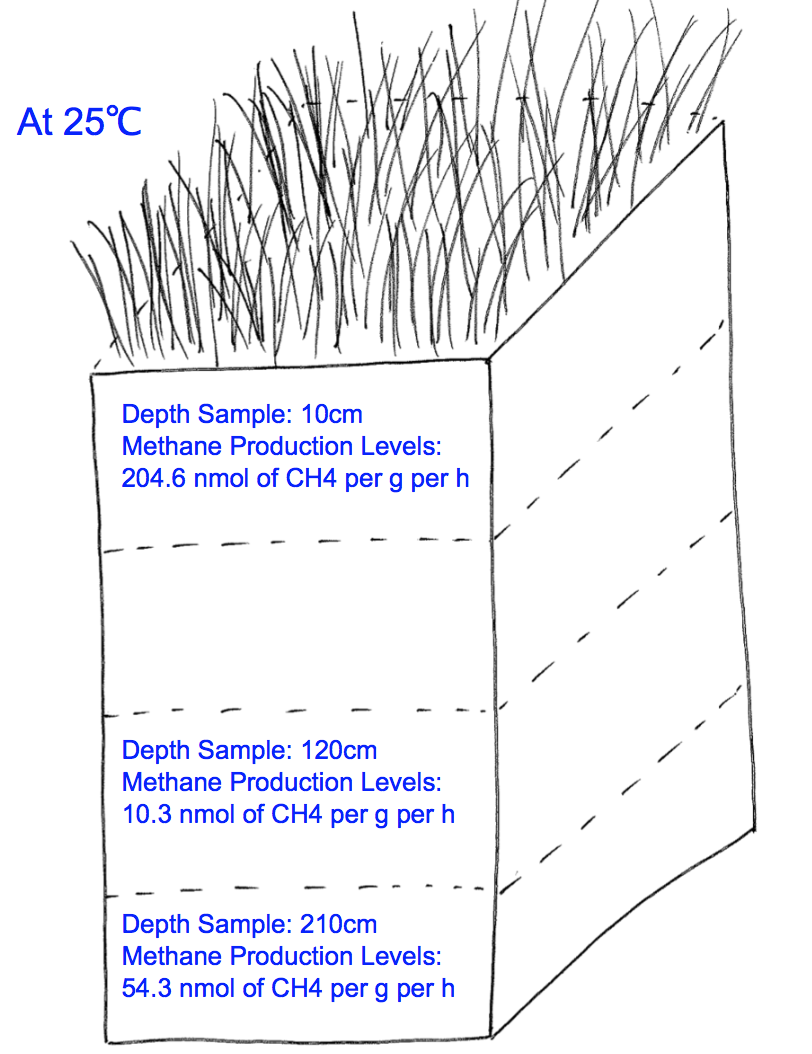
\includegraphics[width=0.75\textwidth]{Methanetemp.png}
  \caption{Effect of temperature on methane production from Cedar Creek peat samples, as published by Richard T. Williams and Ronald L. Crawford in 1984}
  \label{fig:soiltemperature}
\end{figure}

Soil temperature is dependent on two distinct factors --air temperature and artificial human input, such as as prescribed burning. An increase in soil temperature, which increases carbon dioxide levels in peat, has the effect of increasing the fertility of a site \citep{kozlowski2012fire}.

In terms of heat retention, dry humus layers are better at insulation than moist humus layers. The humus layers of artificially burned sites are also more efficient at solar radiation absorbtion, as they are warmer during growth periods as compared to unburned sites \citep{kozlowski2012fire}.

\section{What are the human impacts on peatlands?}

Thus commercialization of peatlands in Southeast Asia has become commonplace with the rise of powerful multinational agribusinesses. Peatlands, as will be discussed in this section, are vulnerable to human-induced fires, climate change, commercialized land use, and more \citep{turetsky2015global}. 

Human impact has led to a multiplicity of current risks in and on peatlands. Firstly, peatlands have become increasingly vulnerable to human-caused burning, especially in tropical regions, as a result of plantation development, agriculture, and logging. Additionally, the rise in human activity has led to an increase in both unintentional and intentional fires, which has made tropical peat prone to excessive burning. This has, in turn, diminished carbon stock. In peatlands of comparatively low latitude, many fire-resistant areas have also become fire prone \citep{turetsky2015global}. The peatlands of low latitude are more likely to have moist microclimates and low-flammability soils. When a peatland is disturbed, however, there is more build-up of dry, flammable fuels and lower humidity because of a reduced tree canopy. 

More significantly, however, rising global temperatures and drainage systems as a result of human activity has led to increasing rates of mineralization. In particular, change in vegetation cover and the use of fertilizers has caused peat to oxidize in the upper peat profile, resulting in increased flux of dissolved organic carbon coupled with elevated levels of greenhouse gas emissions. This means that peatlands, which are originally a long term carbon sink, may actually become carbon emitters that temporarily benefit the economy at the long term detriment of the environment \citep{turetsky2015global}. Increasing greenhouse emission may lead to further rise in global temperatures, further increasing rates of mineralization, constituting a downward vicious spiral.

Unfortunately, in addition to many current risks, Peatlands around the world are also vulnerable to many future risks. Not only are health risks imminent, as a result of respiratory disease and human mortality that is associated with diminished air quality, the thawing of permafrost peatlands may also cause climate change to accelerate. Peat erosion (figure \ref{fig:peaterosion}) in upland temperature peatlands and a decrease in biodiversity may also result \citep{turetsky2015global}. 

\subsection{Climate change}

Anthropogenic climate change can be observed in the regional climate patterns of southeast Asia from the rise of global emissions of carbon dioxide. Climate change can impact seasonal precipitation patterns and there is the potential for peatlands to release stored carbon with the lowering of the water table. This would then create a positive feedback to anthropogenic increases in greenhouse gas emissions but came from drainage affects tree growth. 

As more carbon is released into the atmosphere, the greenhouse effect intensifies. In Southeast Asia, the greenhouse effect and anthropogenic climate change further impacts regional temperature averages. The relationship between the water table and climate change is complex but in peatlands, the plant species suffer from reduced precipitation, one of many impacts of climate change. According to \citet{ahmad2009global}, ''elevated carbon dioxide is expected to decrease stomatal conductance in most species, resulting in less transpiration per unit leaf area.''

In response to rising temperatures, peatlands in the boreal region which are underlain by permafrost are highly unpredictable. In an analysis of peat cores in Canada, the underlying permafrost caused the surface to collapse nearly to the level of the water table \citep{dise2009peatland}. This has profound impacts on the ability of the permafrost to naturally restore itself. 

\citet{holden2005peatland} estimated ``over the past 10,000 years the atmospheric carbon stored in peats has served to reduce global temperatures by about 1.5-2 degrees Celcius.'' 10,000 years on a planetary timescale is a miniscule amount of time. The past hundred years is an even smaller amount of time. Yet, human activity has reversed 10,000 years of carbon sequestration in a few decades. The transformation of peatlands from carbon stores to carbon sources has played a huge role in amplifying anthropogenic climate change. 

Climate change directly impacts plant productivity and the rate of decomposition of organic matter, which is a crucial part of the creation and sustenance of peatlands. Climate change impacts plant productivity in Southeast Asia, which already has warm temperatures, by causing reduced yields and biodiversity. It also impacts the ability of farmers to plan day-to-day operations because the predictability of weather has gone down. Climate change also has indirect effects on peatlands, including changes in hydrology, water balance, and vegetation composition \citep{bonn2016peatland}.

\begin{figure}[!ht]
 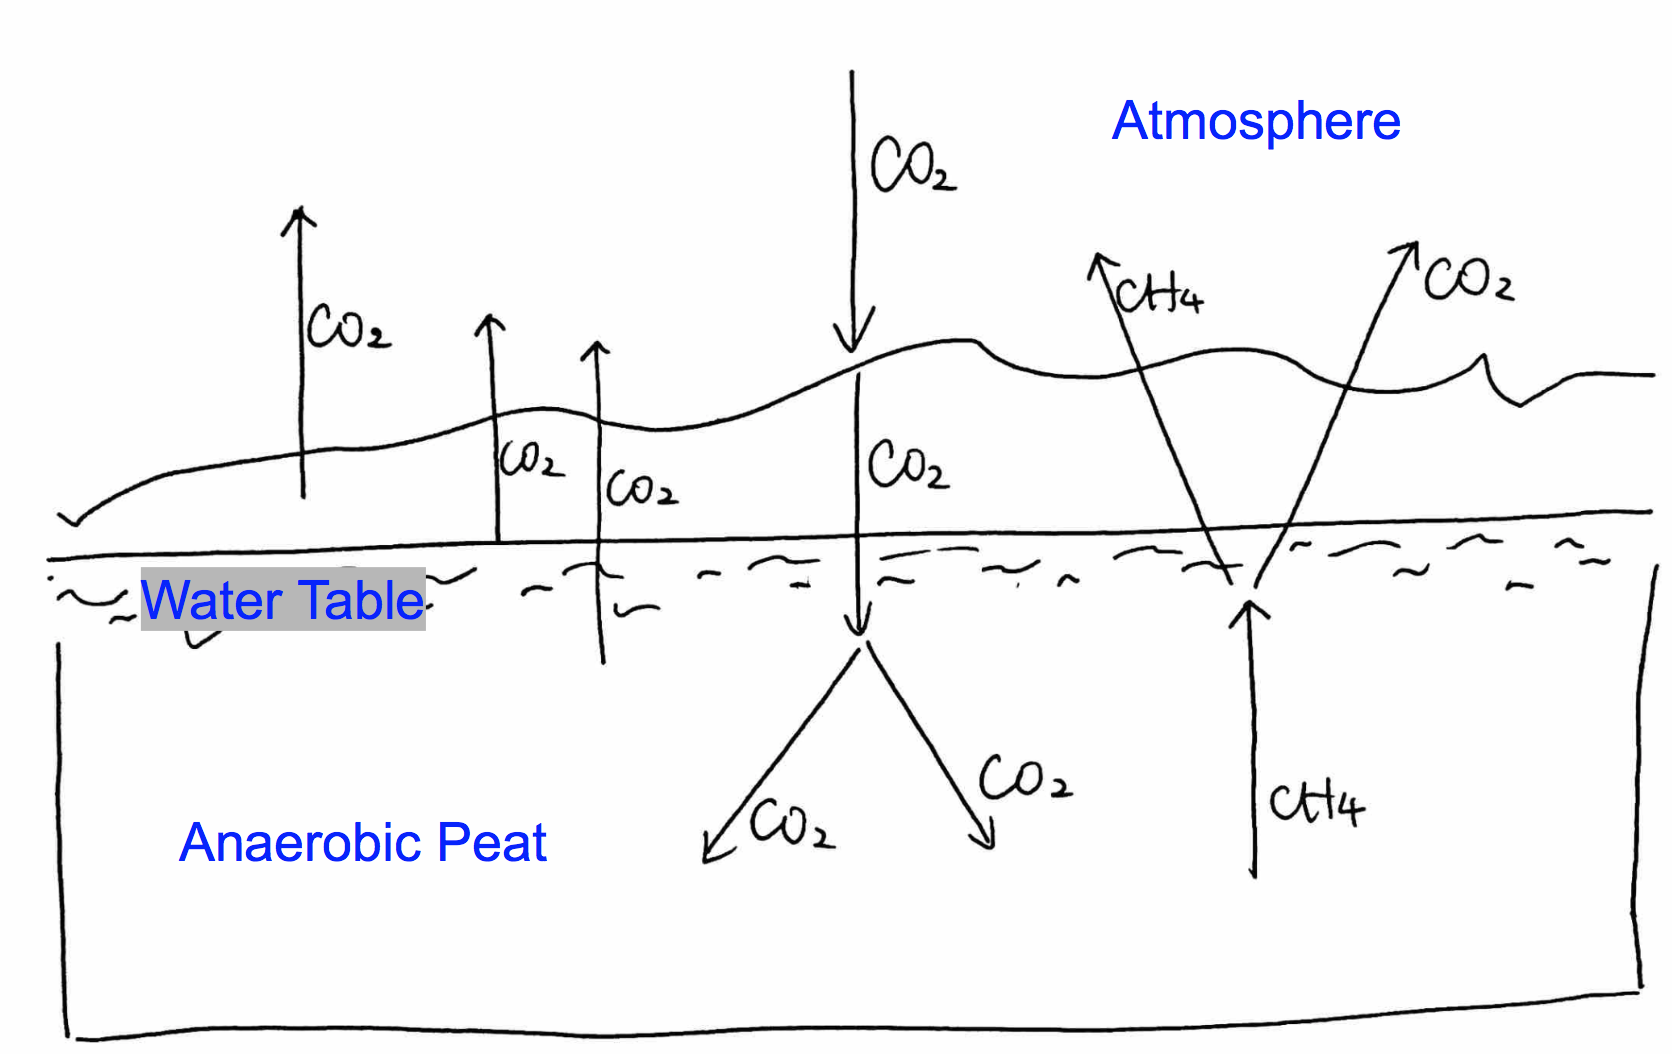
\includegraphics[width=\linewidth]{verticalinterface.png}
  \caption{The vertical interface between peat and the atmosphere: carbon dioxide goes in both directions.}
  \label{fig:peatlandwatertable}
\end{figure}

\subsection{Mineralization}

The greenhouse gas budget of a peatland includes the direct release of carbon dioxide and methane as well as the mineralization of fluvial carbon from dissolved organic carbon and nitrous oxide. Fluvial carbon refers to carbon that is found in rivers. Fluvial carbon has an important role in peatlands in Southeast Asia because the geography of the peatlands is mostly at low altitudes and extend large distances along and between rivers. There are also non-carbon greenhouse gases in the greenhouse gas budget of a peatland that can have varying effects on rising global temperatures, such as nitrous oxide and methane. Carbon, however, is the most common greenhouse gas produced by human activities and the most relevant to peatlands in the region.   

\subsection{Fires}

A large majority of fires in the present day are caused by farmers who want to clear the land and by private corporations that want to create oil palm and pulp wood plantations. Peatlands are particularly vulnerable to fire damage when the forests are cleared and the water table is low after drainage. As a result, fires in peatlands transition from flaming combustion to smouldering combustion. The surface fire burns the vegetation and the smouldering fire burns under the ground, consuming the peat \citep{page2016line}. The smouldering fires burn for very long periods of time and can reignite, even after a short rainy period, depending on changing soil moisture and different levels of peat depth. Below the ground, the low temperature process is under conditions of reduced oxygen availability. This leads to incomplete combustion and intense emissions of direct carbon dioxide and methane as well as the release of toxic compounds like benzene and hydrogen cyanide. 

The number of large-scale fires on peatlands in Southeast Asia has increased greatly over the past couple of decades. Once these peatlands are burned and altered, there is a feedback loop of intensive commercial use, more fires, and the transformation of peatlands into remote swamps. Peatlands that have already been burned once and are either recovering or were only partially burned are then vulnerable to recurrent burning. This repeated burning turns these peatlands into open floodplains with the loss of peat and tree cover. These peatlands are vulnerable to further human activity because the long-term impacts of the fires on health and water quality are difficult to perceive for local communities \citep{chokkalingam2005fire}. The international corporations that contribute to the burning have little incentive to consider the impact on local communities in their commercial process and are not subject to strict regulations that could potentially preserve parts of the peatland or improve ecological health in the region. Because developing economies rely on the profits of billion dollar companies and are much more difficult to regulate, the governments of developing nations struggle to rein in the ecological damage caused by large corporations.

Fire is a tool on industrial plantations because it is much cheaper and quicker to prepare the land this way than by using mechanical technology. Farmers and corporations have little incentive from the state to change methods that are convenient to methods that are better for the environment. In the poor Indonesia Province of Nusa Tenggara Timur (NTT), because fire was an integral part of traditional agricultural practices and because of lack of development in the province, local people have little to zero understanding of modern burning practices and more sustainable fire management problems \citep{russell2007rural}. Problems caused by uncontrolled prescribed burns have deep roots in socioeconomic and cultural differences between developed and undeveloped areas in Southeast Asia. The complexity of these issues and addressing burning practices in a region like Nusa Tenggara Timur, therefore, will require an interdisciplinary approach bringing environmental science, forestry, and anthropology together.  

\begin{figure}[ht]
  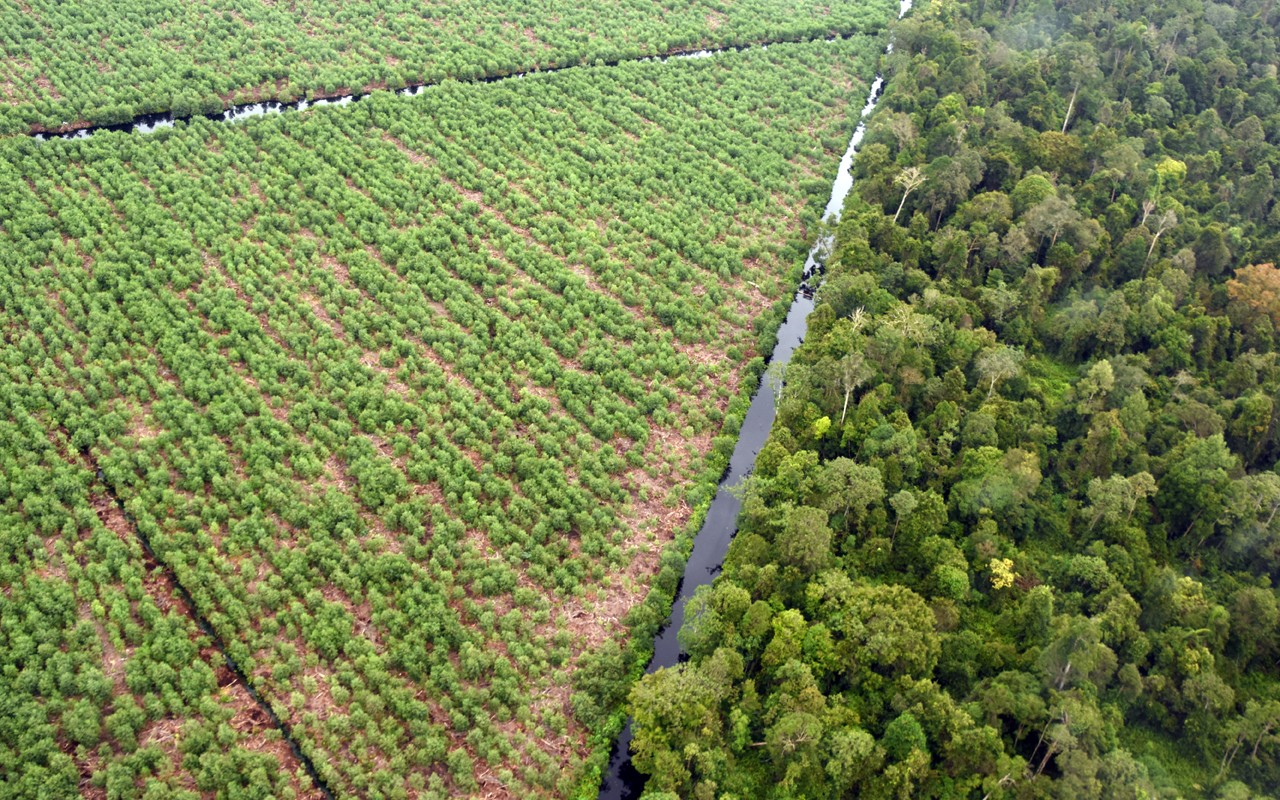
\includegraphics[width=\linewidth]{pulpwoodplantation.jpg}
  \caption{On the left is a pulp wood plantation in Southeast Asia. On the right is what the peatland looked like before being burned and cleared for deforestation. The cultivation of pulp wood on peatlands resembles that of oil palm, especially during this process of preparing the land for monoculture agriculture.}
  \label{fig:pulpwoodplantation}
\end{figure}

\subsection{Land Conversion}

Peatlands are drained to create space for plantations. The drainage happens on land often without regard for the rights of indigenous people who live and rely on the land for survival. The drainage combined with a change in vegetation cover and an intense use of fertilizers leads to peat oxidation in the upper peat profile and increased flux of dissolved organic carbon and increased emissions other greenhouse gases like N2O \citep{larmola2013vegetation}. There are high rates of mineralization, which is the decomposition of chemical compounds in organic matter. Thus, this carbon sink which is built over hundreds of years creates intense short-term carbon emissions. 

Drainage of peatland leads to a large loss of the peat profile and the carbon because aerobic decomposition occurs \citep{page2009restoration}. Peatland drainage leads to peat oxidation and subsidence, which cause the peatland surface to drop to levels that enable the water table to reach and rise above the new surface quicker with high rainfall. This can cause major flooding and expose underlying mineral substrates. 

The global demand for palm oil, which is used in many products, has led to the draining and deforestation of peatland (Figure \ref{fig:peatlanddeforestation}). The story of Arif Subandi, who was forced off his land to make space for oil palm plantations, in the introduction is not uncommon in the region. Palm oil is colloquially referred to as ``green gold'' because Malaysia and Indonesia are the world's largest producers of the agro-industrial commodity \citep{othman2003linking}. Beyond the impacts that draining and deforestation have on peatlands, there are seperate negative impacts of monoculture oil palm plantations which include biodiversity loss, agrochemical runoffs from fertilizers and insecticides, land erosion, and toxic haze, which will be discussed in the next subsection.  

\begin{figure}[ht]
  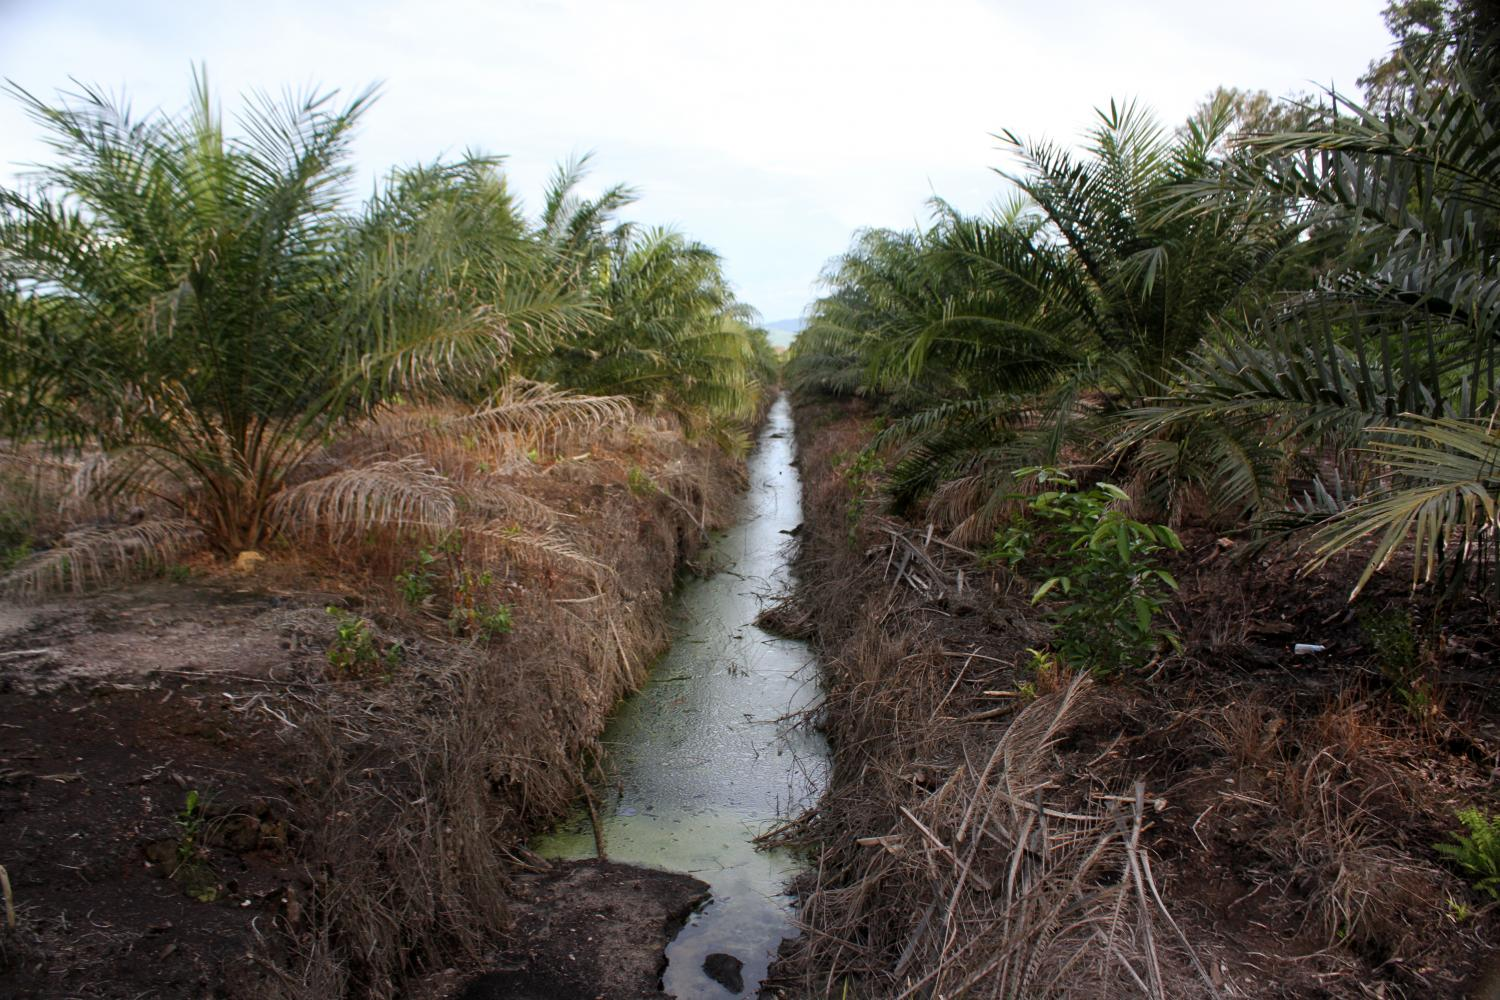
\includegraphics[width=\linewidth]{peatlanddeforestation.jpg}
  \caption{An oil palm plantation created on deforested peatland}
  \label{fig:peatlanddeforestation}
\end{figure}

Peatlands are also subject to the construction of drainage channel and the construction of dams \citep{suyanto2004role}. The dams are constructed for a variety of reasons, such as extracting illegal timber. Another form of direct damage is mining that is done on the peatlands for horticulture and fuel because peat can be an early stage in coal formation, thus making it a significant resource for a nation. 

\section{Indonesian Peatlands Borneo}

Indonesia allows for a concrete examination of peatlands, contributing around 10 to 12 percent of all global peatland resources. In particular, Borneo contains subcoastal peatlands that began to accumulate 22,000 to 23,000 years ago, although, sadly, recent anthropogenic activities have destroyed many of such resources. An example of such would be the burning of peatlands, induced by farmers, in order to establish pulpwood and palm oil plantations, which, though significant to the Indonesian economy, release toxic gases such as aerosols, carbon dioxide, and noxious gases, making Indonesia one of the world's largest greenhouse gas emitters. As of now, extensive deforested and drained peatlands in the region mean vast areas are not only at high risk of accidental ignition, but also cannot be used as farmland \citep{ballhorn2009derivation}.

\section{Conclusion}

The preservation and restoration of peatlands in southeast Asia requires that governments place ecological health over profit from commercialization. There are many global and regional policies that could preserve these vital carbon stocks and thus play an important role in mitigation and adaptation to anthropogenic climate change. As policymakers proceed forward to improve the ecological health of peatlands in Southeast Asia, it is important to keep in mind the need to help local people maintain their livelihoods. Preservation of peatlands will also provide an opportunity for reparations for the injustice done to indigenous peoples. 

The creation of practical programs that can support Southeast Asian countries in preventing fires during El Nino years and drought periods could provide an alternative to the common story of prescribed fires that burn out of control. Peatland restoration has the potential to boost greenhouse gas storage in the soil. Re-wetting the peat manually could play an important role in restoring vegetation and protecting the peat carbon stocks that remain after human alternation. Hydrological restoration could reduce fire risk, though its impact on reducing greenhouse gas emissions is still being studied \citep{page2009restoration}. When thinking about restoration, however, \citet{holden2005peatland} reminds us that we have to ask what we are restoring the peatlands to. Because the climate and environmental conditions today are so different from those that formed peatlands thousands of years ago, ecological restoration for a peatland could look completely different from what we might imagine as "normal." Therefore, we have to continually reexamine what ecological restoration will look like and what a healthy ecosystem looks like in the Anthropocene.

The Katingan Peatland Restoration and Conservation Project is an Borneo-based NGO that is working to help solve the problem by incorporating a business model that offers local people sustainable sources of income. In the Katingan district on the island of Borneo, there is a peat swamp forest that is bigger than Singapore. It is one of the largest remaining intact peat swamp forests left in Indonesia. The project is financed by the sequestration of carbon dioxide and is managed by an Indonesian company, PT. Rimba Makmur Utama. The project is guided by the basic principle that access to the forest will remain open to forest-dependent communities that have traditionally relied on the forest.

An international NGO that is working with local communities in Southeast Asia to preserve peatlands is the Rainforest Action Network, which is California-based (figure \ref{fig:ranpalmoil}). Where Katingan Peatland Restoration and Conservation Project is focused on providing on-the-ground solutions, the Rainforest Action Network works with the large international corporations that own the largest plantations in Southeast Asia for oil palm and wood pulp. Their aim is to encourage economic, social, and environmental sustainability within the supply chains of corporations like PepsiCo and General Mills.

\begin{figure}{!ht}
  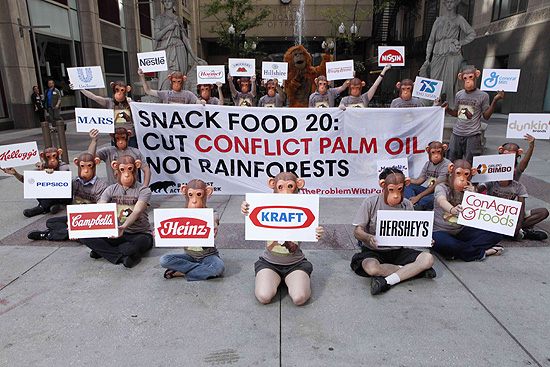
\includegraphics[width=\linewidth]{ranpalmoil.jpg}
  \caption{A protest by Rainforest Action Network activists demanding that international corporations preserve peatlands and rainforests.}
  \label{fig:ranpalmoil}
\end{figure}

Another potential solution to peatland restoration, and thus greater planetary health, is in biomimcry. Biomimicry is the design of materials, structures, and systems that are inspired by biological processes. Biomimicry is a relatively new framework of thinking but it could be used to facilitate the creation of peatlands, which usually takes thousands and thousands of years. A question to be explored is how biomimicry can be used to improve soil quality and soil temperature. In this way, we can maintain human activity sustainably and ecological health. The two are not mutually exclusive.  

Finally, though peatlands like all other natural lands are threatened by human activity, \citet{dise2009peatland} says that peatlands are complex adaptive systems that are "resilient to change at some level of pertubation but shifting to new states at higher levels of disturbance." We must not ignore the valuable signals from the anthropogenic changes in peatlands that we are seeing now but we must also remember that peatlands, like the planet, are resilient.  

